% beamer_template.tex
% 2014-06-18 dmontaner@cipf.es
% Beamer template. Ready to use with pandoc

% For templates see:
% http://deic.uab.es/~iblanes/beamer_gallery/
% For colors see:
% http://deic.uab.es/~iblanes/beamer_gallery/index_by_color.html

%% Latex themes seem to be stored here:
%% /usr/share/texmf/tex/latex/beamer/base/themes

%% tree /usr/share/texmf/tex/latex/beamer/base/themes
%% ├── color
%% │   ├── beamercolortheme...albatross.sty
%% │   ├── beamercolortheme...beaver.sty
%% │   ├── beamercolortheme...beetle.sty
%% │   ├── beamercolortheme...crane.sty
%% │   ├── beamercolortheme...default.sty
%% │   ├── beamercolortheme...dolphin.sty
%% │   ├── beamercolortheme...dove.sty
%% │   ├── beamercolortheme...fly.sty
%% │   ├── beamercolortheme...lily.sty
%% │   ├── beamercolortheme...monarca.sty
%% │   ├── beamercolortheme...orchid.sty
%% │   ├── beamercolortheme...rose.sty
%% │   ├── beamercolortheme...seagull.sty
%% │   ├── beamercolortheme...seahorse.sty
%% │   ├── beamercolortheme...sidebartab.sty
%% │   ├── beamercolortheme...spruce.sty
%% │   ├── beamercolortheme...structure.sty
%% │   ├── beamercolortheme...whale.sty
%% │   └── beamercolortheme...wolverine.sty
%% ├── font
%% │   ├── beamerfonttheme...default.sty
%% │   ├── beamerfonttheme...professionalfonts.sty
%% │   ├── beamerfonttheme...serif.sty
%% │   ├── beamerfonttheme...structurebold.sty
%% │   ├── beamerfonttheme...structureitalicserif.sty
%% │   └── beamerfonttheme...structuresmallcapsserif.sty
%% ├── inner
%% │   ├── beamerinnertheme...circles.sty
%% │   ├── beamerinnertheme...default.sty
%% │   ├── beamerinnertheme...inmargin.sty
%% │   ├── beamerinnertheme...rectangles.sty
%% │   └── beamerinnertheme...rounded.sty
%% ├── outer
%% │   ├── beameroutertheme...default.sty
%% │   ├── beameroutertheme...infolines.sty
%% │   ├── beameroutertheme...miniframes.sty
%% │   ├── beameroutertheme...shadow.sty
%% │   ├── beameroutertheme...sidebar.sty
%% │   ├── beameroutertheme...smoothbars.sty
%% │   ├── beameroutertheme...smoothtree.sty
%% │   ├── beameroutertheme...split.sty
%% │   └── beameroutertheme...tree.sty
%% └── theme
%%     ├── beamertheme...AnnArbor.sty
%%     ├── beamertheme...Antibes.sty
%%     ├── beamertheme...Bergen.sty
%%     ├── beamertheme...Berkeley.sty
%%     ├── beamertheme...Berlin.sty
%%     ├── beamertheme...Boadilla.sty
%%     ├── beamertheme...boxes.sty
%%     ├── beamertheme...CambridgeUS.sty
%%     ├── beamertheme...Copenhagen.sty
%%     ├── beamertheme...Darmstadt.sty
%%     ├── beamertheme...default.sty
%%     ├── beamertheme...Dresden.sty
%%     ├── beamertheme...EastLansing.sty
%%     ├── beamertheme...Frankfurt.sty
%%     ├── beamertheme...Goettingen.sty
%%     ├── beamertheme...Hannover.sty
%%     ├── beamertheme...Ilmenau.sty
%%     ├── beamertheme...JuanLesPins.sty
%%     ├── beamertheme...Luebeck.sty
%%     ├── beamertheme...Madrid.sty
%%     ├── beamertheme...Malmoe.sty
%%     ├── beamertheme...Marburg.sty
%%     ├── beamertheme...Montpellier.sty
%%     ├── beamertheme...PaloAlto.sty
%%     ├── beamertheme...Pittsburgh.sty
%%     ├── beamertheme...Rochester.sty
%%     ├── beamertheme...Singapore.sty
%%     ├── beamertheme...Szeged.sty
%%     ├── beamertheme...Warsaw.sty
%%     └── compatibility
%%         ├── beamertheme...bars.sty
%%         ├── beamertheme...classic.sty
%%         ├── beamertheme...compatibility.sty
%%         ├── beamertheme...lined.sty
%%         ├── beamertheme...plain.sty
%%         ├── beamertheme...shadow.sty
%%         ├── beamertheme...sidebar.sty
%%         ├── beamertheme...split.sty
%%         └── beamertheme...tree.sty


%% Inner Themes
%% =============================================================================

%% An inner theme installs templates that dictate how the following elements 
%% are typeset:
%% - Title and part pages.
%% - Itemize environments.
%% - Enumerate environments.
%% - Description environments.
%% - Block environments.
%% - Theorem and proof environments.
%% - Figures and tables.
%% - Footnotes.
%% - Bibliography entries.

%% Outer Themes
%% =============================================================================
%% An outer theme dictates the overall layout of frames. 
%% It specifies where any navigational elements should go 
%% and what they should look like. 

%% An outer theme specifies how the following elements are rendered:
%% - The head- and footline.
%% - The sidebars.
%% - The logo.
%% - The frame title.

%%%%%%%%%%%%%%%%%%%%%%%%%%%%%%%%%%%%%%%%%%%%%%%%%%%%%%%%%%%%%%%%%%%%%%%%%%%%%%%%
%%% TEMPLATE
%%%%%%%%%%%%%%%%%%%%%%%%%%%%%%%%%%%%%%%%%%%%%%%%%%%%%%%%%%%%%%%%%%%%%%%%%%%%%%%%

%% Document
\documentclass{beamer}
\usepackage[utf8]{inputenc}
\usepackage[T1]{fontenc} % Spanish characters
\usepackage{lmodern}     % Use always with T1. Otherwise the letter looks weird.
%\usepackage{graphicx}   % ??? SEE WHY IS NOT ON

%% TABLES
\usepackage{longtable,booktabs}        % the package is needed in Pandoc
\usepackage{caption}
\makeatletter                          % These lines are needed 
\def\fnum@table{\tablename~\thetable}  % to make table captions 
\makeatother                           % work with longtable.


%%%%%%%%%%%%%%%%%%%%%%%%%%%%%%%%%%%%%%%%%%%%%%%%%%%%%%%%%%%%%%%%%%%%%%%%%%%%%%%%
%%% PARAMETERS (has to be here: after the utf8 encoding)
%%%%%%%%%%%%%%%%%%%%%%%%%%%%%%%%%%%%%%%%%%%%%%%%%%%%%%%%%%%%%%%%%%%%%%%%%%%%%%%%

%% \def \titulolargo {This is my LONG title} % long title:  this will go to the FIRST slide.
%% \def \titulocorto {short title}           % short title: this will go to the FOOTER of the slides.
%% \def \subtitulo {my subtitle}
%% \def \autorlargo {David Montaner} % long author:  this will go to the FIRST slide.
%% \def \autorcorto {D. Montaner}    % short author: this will go to the FOOTER of the slides.
%% \def \fecha {mifecha 2014-06-18}


%% to be used as a pandoc template
\def \titulolargo {NGS Data Analysis Course}         % long title:  this will go to the FIRST slide.
\def \titulocorto {NGS Data Analysis Course}  % short title: this will go to the FOOTER of the slides.
\def \subtitulo {Association Analysis using PLINK}
\def \autorlargo {Marta Bleda, Javier Lopez, Ignacio Medina, David Montaner}         % long author:  this will go to the FIRST slide.
\def \autorcorto {Association Analysis}    % short author: this will go to the FOOTER of the slides.
\def \fecha {2015-02-22}
\def \pagina {http://www.ngscourse.org}


%% My Beamer Combinations %%%%%%%%%%%%%%%%%%%%%%%%%%%%%%%%%%%%%%%%%%%%%%%%%%%%%%

%% % Orange
%% \useinnertheme[shadow]{rounded}
%% \usecolortheme{crane}
%% \useoutertheme{shadow}  % INCLUDES THE FOOTER

% Light blue
\useinnertheme[shadow]{rounded}
\usecolortheme{seahorse}
\useoutertheme{shadow}  % INCLUDES THE FOOTER

% Strong blue
%% \useinnertheme[shadow]{rounded}
%% \usecolortheme{whale}
%% \useoutertheme{shadow}  % INCLUDES THE FOOTER

%%%%%%%%%%%%%%%%%%%%%%%%%%%%%%%%%%%%%%%%%%%%%%%%%%%%%%%%%%%%%%%%%%%%%%%%%%%%%%%%


%% beamer theme INNER
%\useinnertheme{default}
%\useinnertheme{rectangles} %squared bullets
%\useinnertheme{circles}    %circular bullets
%\useinnertheme{rounded}         % bullets as balls, round borders                               FAVORITE ; use with seahorse and whale
%\useinnertheme[shadow]{rounded} % bullets as balls, round borders and shadow under the boxes    FAVORITE ; do not use with seahorse or whale


%% beamer theme OUTER
%\useoutertheme{default}
%\useoutertheme{infolines} % with slide number but I do not like it. It has also sections. The title is short.
%\useoutertheme{split}  
%\useoutertheme{shadow}    % INCLUDES THE FOOTER


%% beamer COLOR
%% SEE http://deic.uab.es/~iblanes/beamer_gallery/index_by_color.html

%\usecolortheme{whale}     % dark blue             FAVORITE
%\usecolortheme{seahorse}  % light blue            FAVORITE
%\usecolortheme{crane}     % orange and squared    FAVORITE

%\usecolortheme{default}
%\usecolortheme{orchid}    % white background
%\usecolortheme{dove}      % white background and black titles. Not nice boxes
%\usecolortheme{rose}      % white background; blocks are OK in blue
%\usecolortheme{wolverine} % orange yellow; no squares
%\usecolortheme{fly}       % gray Background
%\usecolortheme{beetle}    % gray Background and blue titles. Not very interesting.


%% beamer FONT
%\usefonttheme{default}      % sans serif font f
\usefonttheme{structurebold} % nice font (I do not know which is it)


% beamer EXTRA options (set them after the theme)
\setbeamertemplate{frametitle}[default][center] % centering titles
\setbeamertemplate{navigation symbols}{}        % suppresses all navigation symbols

\setbeamertemplate{caption}{\insertcaption}     % suppresses the 'Figure' tagging in images
\setbeamertemplate{caption label separator}{}


%%%%%%%%%%%%%%%%%%%%%%%%%%%%%%%%%%%%%%%%%%%%%%%%%%%%%%%%%%%%%%%%%%%%%%%%%%%%%%%%

%%% GENERAL SETTINGS

%% Color links
\definecolor{links}{HTML}{2A1B81}                  % color for links SEE IF THEY WORK WITH ALL THEMES: 'whale', 'seahorse' and 'crane'.
\hypersetup{colorlinks,linkcolor=,urlcolor=links}

%% Color verbatim
\makeatletter 
\renewcommand\verbatim@font{\normalfont\ttfamily\color{violet}}  % not too bad for all my theme combinations.
%\renewcommand\verbatim@font{\normalfont\ttfamily\color{orange}}
%\renewcommand\verbatim@font{\normalfont\ttfamily\color{blue}}
%\renewcommand\verbatim@font{\normalfont\ttfamily\color{green}}
%\renewcommand\verbatim@font{\normalfont\ttfamily\color{gray}}
%\renewcommand\verbatim@font{\normalfont\ttfamily\color{red}}
%\renewcommand\verbatim@font{\normalfont\ttfamily\color{pink}}
\makeatother

%% % Scale images as in the pandoc template
%% % WORKS but if used 'scale' DOES NOT WORK
%% \usepackage{graphicx}
%% \makeatletter
%% \def \maxwidth  {\ifdim \Gin@nat@width  > \linewidth     \linewidth    \else \Gin@nat@width  \fi}
%% \def \maxheight {\ifdim \Gin@nat@height > \textheight   0.8\textheight \else \Gin@nat@height \fi}
%% \makeatother
%% % Scale images if necessary, so that they will not overflow the page
%% % margins by default, and it is still possible to overwrite the defaults
%% % using explicit options in \includegraphics[width, height, ...]{}
%% \setkeys{Gin}{width=\maxwidth,height=\maxheight,keepaspectratio}

%% Separation between paragraphs
%\setlength{\parskip}{\baselineskip}
%\parskip=1.5ex % ex is a vertical measure

%% Bullet separation from previous paragraph: IMPOSSIBLE
%% see: <http://tex.stackexchange.com/questions/115907/how-do-i-remove-white-space-above-itemize-command-in-beamer-using-enumitem>
%% It's not a good idea to use the enumitem package with beamer since beamer has its own ways of dealing with the standard list-like environment
%\usepackage{enumitem}
%\setlist[itemize]{noitemsep, topsep=0pt, partopsep=0pt}



%%%%%%%%%%%%%%%%%%%%%%%%%%%%%%%%%%%%%%%%%%%%%%%%%%%%%%%%%%%%%%%%%%%%%%%%%%%%%%%%
%% TITLE (depends on definde parameters)
%%%%%%%%%%%%%%%%%%%%%%%%%%%%%%%%%%%%%%%%%%%%%%%%%%%%%%%%%%%%%%%%%%%%%%%%%%%%%%%%
\title[{\makebox[.45\paperwidth]{\titulocorto \hfill \insertframenumber/\inserttotalframenumber}}]{\titulolargo}
\subtitle{{\color{gray}\subtitulo}}  %% GREY is nice for the 'whale', 'seahorse' and the 'crane' color themes
%\subtitle{\subtitulo}

\author[\autorcorto]{\autorlargo}

\date{\fecha \newline \newline \url{\pagina}}


%%%%%%%%%%%%%%%%%%%%%%%%%%%%%%%%%%%%%%%%%%%%%%%%%%%%%%%%%%%%%%%%%%%%%%%%%%%%%%%%
%% DOCUMENT %%%%%%%%%%%%%%%%%%%%%%%%%%%%%%%%%%%%%%%%%%%%%%%%%%%%%%%%%%%%%%%%%%%%
%%%%%%%%%%%%%%%%%%%%%%%%%%%%%%%%%%%%%%%%%%%%%%%%%%%%%%%%%%%%%%%%%%%%%%%%%%%%%%%%
\begin{document}

%% title frame
\begin{frame}
  \maketitle
\end{frame}

\begin{frame}{File formats: VCF}

Tab delimited text file with a \textbf{header section}

~

\centerline{\includegraphics[scale=0.35]{images/vcf.png}}

~

May be compressed and indexed using \texttt{tabix}

\end{frame}

\begin{frame}{File formats: VCF}

Each variant is described by \textbf{8 fields}

\begin{enumerate}
\def\labelenumi{\arabic{enumi}.}
\item
  CHROM: chromosome
\item
  POS: position
\item
  ID: name
\item
  REF: reference base(s)
\item
  ALT: non-reference alleles
\item
  QUAL: quality score of the calls (phred scale)
\item
  FILTER: PASS / filtering\_tag
\item
  INFO: additional information
\end{enumerate}

\textbf{Genotype data} for several samples may be included in a batch of
additional columns (one for each sample) preceded by a FORMAT column
which describes their format.

\end{frame}

\begin{frame}[fragile]{File formats: VCF INFO column}

May include several semicolon separated fields containing information
about the variants coded in key value style:

\begin{verbatim}
<key>=<data>[,data]
\end{verbatim}

Some reserved (but optional) keys are:

\begin{itemize}
\itemsep1pt\parskip0pt\parsep0pt
\item
  AA ancestral allele
\item
  AC allele count in genotypes, for each ALT allele, in the same order
  as listed
\item
  AF allele frequency
\item
  CIGAR cigar string describing how to align an alternate allele to the
  reference allele
\item
  DB dbSNP membership
\item
  MQ RMS mapping quality, e.g.~MQ=52
\item
  MQ0 Number of MAPQ == 0 reads covering this record
\end{itemize}

\end{frame}

\begin{frame}{File formats: PED \& MAP}

Classic format to represent genomic variants for several individuals

\centerline{\includegraphics[scale=0.3]{images/ped-map.png}}

\end{frame}

\begin{frame}{File formats: PED \& MAP}

\begin{block}{PED file}

\begin{enumerate}
\def\labelenumi{\arabic{enumi}.}
\itemsep1pt\parskip0pt\parsep0pt
\item
  Family ID
\item
  Individual ID
\item
  Paternal ID
\item
  Maternal ID
\item
  Sex (1=male; 2=female; other=unknown)
\item
  Phenotype (1=unaffected; 2=affected; 0 missing; -9=missing)
\item
  \ldots{} genotypes \ldots{}
\end{enumerate}

\end{block}

\begin{block}{MAP file}

\begin{enumerate}
\def\labelenumi{\arabic{enumi}.}
\itemsep1pt\parskip0pt\parsep0pt
\item
  chromosome (1-22, X, Y or 0 if unplaced)
\item
  rs\ldots{} or SNP identifier
\item
  Genetic distance (Morgans)
\item
  Base-pair position (bp units)
\end{enumerate}

\end{block}

\end{frame}

\begin{frame}{Association to Disease / Phenotype}

\centerline{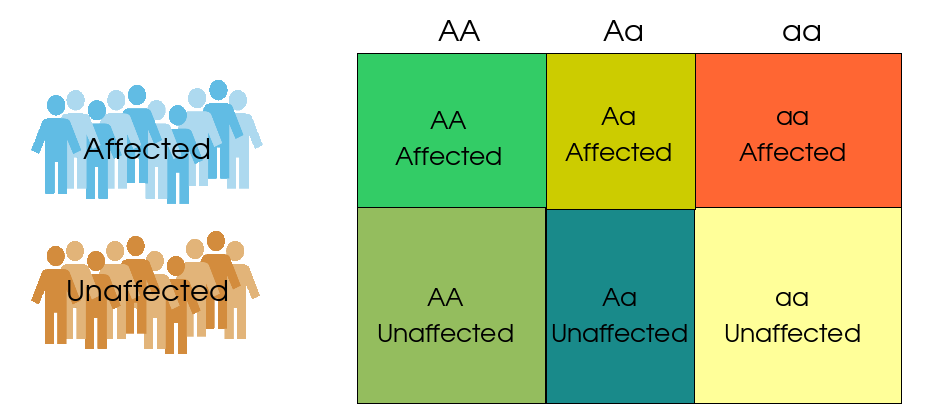
\includegraphics[scale=0.3]{images/asoc_table_3.png}}

\begin{longtable}[c]{@{}rccc@{}}
\toprule
~ & AA & Aa & aa\tabularnewline
\midrule
\endhead
Affected & 15 & 8 & 4\tabularnewline
Unaffected & 5 & 3 & 2\tabularnewline
\bottomrule
\end{longtable}

30+8 \textbar{} 8+8

10+3 \textbar{} 3+4

\end{frame}

\begin{frame}{Association to Disease / Phenotype}

\centerline{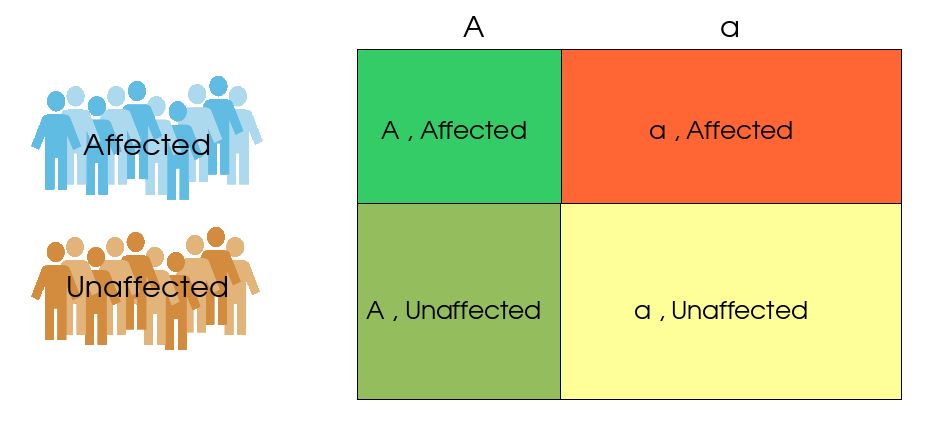
\includegraphics[scale=0.3]{images/asoc_table_2.png}}

\begin{longtable}[c]{@{}rcc@{}}
\toprule
~ & A & a\tabularnewline
\midrule
\endhead
Affected & 38 & 16\tabularnewline
Unaffected & 13 & 7\tabularnewline
\bottomrule
\end{longtable}

\end{frame}

\begin{frame}{Statistical tests}

\begin{itemize}
\itemsep1pt\parskip0pt\parsep0pt
\item
  \href{http://en.wikipedia.org/wiki/Chi-squared_test}{Chi-squared test}
  (\(\chi^2\))
\item
  \href{http://en.wikipedia.org/wiki/Fisher's_exact_test}{Fisher's
  exact}
\item
  \href{http://en.wikipedia.org/wiki/Logistic_regression}{Logistic
  regression models}
\item
  \ldots{}
\end{itemize}

\href{http://www.ncbi.nlm.nih.gov/pmc/articles/PMC2907892/}{Multiple-test
correction} is generally needed.

Many software available \href{http://cran.es.r-project.org/}{R},
\href{http://pngu.mgh.harvard.edu/~purcell/plink/}{PLINK} \ldots{}

\url{http://pngu.mgh.harvard.edu/~purcell/plink/anal.shtml}

\end{frame}

%% %%%%%%%%%%%%%%%%%%%%%%%%%%%%%%%%%%%%%%%%%%%%%%%%%%%%%%%%%%%%

%% \begin{frame}
%%   \frametitle{Titulo}
%%   \framesubtitle{SubTitulo}
  
%%   \begin{itemize}
%%   \item uno
%%   \item dos
%%   \end{itemize}  

%%   \url{http://www.dmontaner.com/}

%%   \href{http://www.dmontaner.com/}{un link}

%%   \begin{enumerate}
%%   \item uno número
%%   \item dos número
%%   \end{enumerate}  

%% \end{frame}

%% %%%%%%%%%%%%%%%%%%%%%%%%%%%%%%%%%%%%%%%%%%%%%%%%%%%%%%%%%%%%

%% \begin{frame}[fragile]
%%   \frametitle{Verbatim}
  
%%   Este es un texto en \texttt{verbatim}
  
%%   \begin{verbatim}

%%     ver si no sera mejor ponerle un background
    
%%     texto o codigo tal cual 
%%     texto o codigo  tal cual hasta con espacios
    
%%   \end{verbatim}
  
%% \end{frame}

%% %%%%%%%%%%%%%%%%%%%%%%%%%%%%%%%%%%%%%%%%%%%%%%%%%%%%%%%%%%%%

%% \begin{frame}
%%   \frametitle{Parrafos}

%%   PRIMER PARRAFO: Don Juan Carlos, de 76 años, se ha dirigido a la nación a través 
%%   de la televisión pública para explicar los motivos de su renuncia: 
  
%%   AQUI EMPIEZA EL SEGUNDO PARRAFO: "Hoy merece pasar a la primera línea una generación 
%%   más joven, con nuevas energías y con una nueva forma de enfrentar la realidad".
  
  
%%   \begin{itemize}
%%   \item uno
%%   \item dos
%%   \end{itemize}  
  
%%   AQUI EMPIEZA EL TERCER PARRAFO: El Rey ha agradecido su ayuda a la Reina durante 
%%   todos estos años; ha dicho que el Príncipe Felipe cuenta con la "madurez, 
%%   la preparación y el compromiso necesarios" para ser el próximo jefe del Estado,
%%   y ha recordado que éste cuenta con "el apoyo de la Princesa Letizia".

%% \end{frame}

%% %%%%%%%%%%%%%%%%%%%%%%%%%%%%%%%%%%%%%%%%%%%%%%%%%%%%%%%%%%%%

%% \begin{frame}
%%   \frametitle{Images: big}
%%   \includegraphics[width=\textwidth,height=0.8\textheight,keepaspectratio]{images/big}
%% \end{frame}

%% \begin{frame}
%%   \frametitle{Images: small}
%%   \includegraphics[width=\textwidth,height=0.8\textheight,keepaspectratio]{images/small}
%% \end{frame}

%% %%%

%% \begin{frame}
%%   \frametitle{Images: big SCALED}
%%   \includegraphics[width=\textwidth,height=0.8\textheight,keepaspectratio]{images/big}
%% \end{frame}

%% \begin{frame}
%%   \frametitle{Images: small SCALED}
%%   \includegraphics[width=\textwidth,height=0.8\textheight,keepaspectratio]{images/small}
%% \end{frame}

%% %%%

%% \begin{frame}
%%   \frametitle{Images: big RE-SCALED}
%%   \includegraphics[scale=0.1]{images/big}
%% \end{frame}

%% %%%%%%%%%%%%%%%%%%%%%%%%%%%%%%%%%%%%%%%%%%%%%%%%%%%%%%%%%%%%

%% \begin{frame}
%%   \frametitle{Bloques}
  
%%   Van los bloques a ver como se organizan.

%%   \begin{block}{Bloque uno}
%%     una cosa aqui dentro
%%   \end{block}


%%   \begin{block}{Otro bloque}
%%     \begin{itemize}
%%     \item uno
%%     \item dos
%%     \end{itemize}  
%%   \end{block}

%%   Con una linea de separacion

%%   \begin{block}{Bloque uno}
%%     otra cosa aqui dentro
%%   \end{block}

%%   Y fuera del utlimo bloque

%% \end{frame}

%% %%%%%%%%%%%%%%%%%%%%%%%%%%%%%%%%%%%%%%%%%%%%%%%%%%%%%%%%%%%%

%% \begin{frame}
%%   \frametitle{Cosita}
  
%%   Que hace esto

%%   ~ 

%%   parece que deja un doble espacio entre parrafos

%%   de todo

%% \end{frame}



%%%%%%%%%%%%%%%%%%%%%%%%%%%%%%%%%%%%%%%%%%%%%%%%%%%%%%%%%%%%%%%%%%%%%%%%%%%%%%%%
%% DOCUMENT END %%%%%%%%%%%%%%%%%%%%%%%%%%%%%%%%%%%%%%%%%%%%%%%%%%%%%%%%%%%%%%%%
\end{document}
